\section{Experimental design}
\subsection{Systems and primary operating points}
The dense reference is AudioLDM-M-Full~\cite{liu2023audioldm}, with $415.96$\,M U-Net parameters. We study two released pruning severities~\cite{singh2026pruning}. Severity~1 retains $145.67$\,M parameters, corresponding to $65.0\%$ pruning. Severity~2 retains $71.08$\,M, corresponding to $82.9\%$ pruning. At each severity, P denotes the checkpoint before recovery and \PFT{} the released checkpoint after $10^{6}$ AudioCaps fine-tuning steps. Their paired difference isolates the gain of that recovery stage within the pruned architecture. It does not isolate an effect caused by pruning relative to a dense model given the same fine-tune.

The primary duration comparison uses $3.84$ and $10.24$\,s. Severity~2 adds $5.12$ and $7.68$\,s, yielding a four-point sweep. The original in-domain battery uses AudioCaps \textsc{test}~\cite{kim2019audiocaps}. The extreme held-out battery uses hip-hop and rap captions from MusicCaps~\cite{agostinelli2023musiclm}. Primary severity~2 inference uses $192$ AudioCaps prompts and the original hip-hop battery uses $64$ prompts. Severity~1 originally uses $80$ prompts for duration.

Generation uses DDIM~\cite{song2021ddim} with $50$ steps, guidance $2.5$ and $\eta=0$. A pre-specified robustness check repeats the severity~2 endpoint comparison with the published DDIM $200$, guidance $3.5$ recipe.

\subsection{Mechanism and boundary checks}
The follow-up experiments were designed after the original analyses and frozen before their own generation and scoring. They are reported as mechanism and boundary-condition checks rather than as part of the original confirmatory family.

Three checks address duration. First, we fine-tune the severity~2 pruned checkpoint for $20{,}000$ steps using $3.84$\,s random AudioCaps crops and then evaluate that checkpoint at both $3.84$ and $10.24$\,s. If the duration interaction reflects specialization to the training duration, this intervention should reverse its direction. Second, a public dense AudioLDM-M text-fine-tuned checkpoint provides a non-matched reference for whether duration-dependent fine-tuning gains occur without pruning. Third, we extend the released recovery sweep to $15.36$\,s on $96$ prompts. We also add $96$ new severity~1 prompts, increasing the pooled duration sample to $176$.

The domain follow-up adds Clotho~\cite{drossos2020clotho}, with $96$ clips selected before scoring. Its captions are closer in length to AudioCaps than the hip-hop captions, while the dataset remains held out from recovery. We also generate dense references for the hip-hop cells and extend that battery from $64$ to $127$ prompts. These two checks separate a weak recovery effect from a battery that is simply unable to discriminate text-audio alignment.

\subsection{Pairing, endpoints and estimands}
Within an operating point, P and \PFT{} receive identical diffusion noise $x_T$ for each prompt. This common-random-number design removes a large source of sampling variance from the paired difference. The prompt is the statistical unit. Replicates are averaged within prompt before inference, and $95\%$ intervals use a prompt-level percentile bootstrap with $B=10^{4}$ resamples.

The primary endpoint is fused CLAP cosine from \texttt{laion/\allowbreak clap-htsat-fused}, revision \texttt{365dea6e}~\cite{wu2023clap}. A shuffled-caption floor pairs each clip with captions from other prompts in the same battery. Matched dense generations provide a model reference, and real AudioCaps or Clotho recordings provide a data reference when available.

For operating point $o$, recovery gain is
\begin{equation}
R(o)=\mathbb{E}_{i}\left[S(\PFT,i,o)-S(P,i,o)\right].
\end{equation}
The duration interaction is $J=R(10.24\,\mathrm{s})-R(3.84\,\mathrm{s})$. A positive $J$ means that recovery itself is larger at the longer operating point. We also report
\begin{equation}
\rho_{\mathrm{ref}}=\frac{R}{S(\mathrm{ref})-S(P)},
\end{equation}
which expresses the gain as a fraction of the available gap to a reference.

The original severity~2 duration and domain contrasts and the published-sampler check were specified before their corresponding scores were computed. The four-duration sweep was registered after the primary result but before its own scoring. Human-CLAP, KL, PANNs, anchor decomposition and crop analysis are corroborative or diagnostic analyses and are interpreted accordingly.

\begin{figure*}[t]
\centering
\begin{minipage}[t]{0.49\textwidth}
\centering
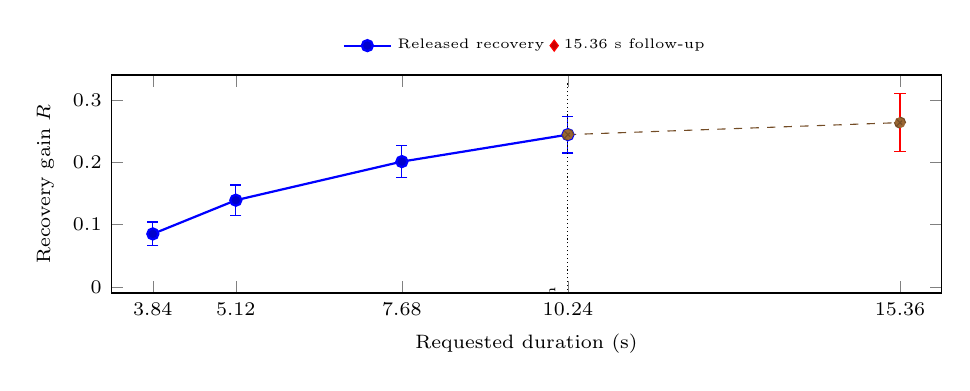
\begin{tikzpicture}
\begin{axis}[
width=\linewidth,height=4.35cm,
xlabel={Requested duration (s)},
ylabel={Recovery gain $R$},
xmin=3.2,xmax=16.0,ymin=-0.01,ymax=0.34,
xtick={3.84,5.12,7.68,10.24,15.36},
xticklabels={3.84,5.12,7.68,10.24,15.36},
tick label style={font=\scriptsize},label style={font=\scriptsize},
legend style={font=\tiny,draw=none,fill=none,at={(axis description cs:0.5,1.05)},anchor=south,legend columns=-1}]
\addplot+[mark=*,thick,error bars/.cd,y dir=both,y explicit]
coordinates {(3.84,0.0849) +- (0,0.0191) (5.12,0.139) +- (0,0.0245) (7.68,0.201) +- (0,0.026) (10.24,0.2443) +- (0,0.0295)};
\addlegendentry{Released recovery}
\addplot+[mark=diamond*,only marks,error bars/.cd,y dir=both,y explicit]
coordinates {(15.36,0.2636) +- (0,0.0471)};
\addlegendentry{$15.36$ s follow-up}
\addplot+[dashed,forget plot] coordinates {(10.24,0.2443) (15.36,0.2636)};
\draw[densely dotted] (axis cs:10.24,-0.005) -- (axis cs:10.24,0.33);
\node[font=\tiny,rotate=90,anchor=south east] at (axis cs:10.24,0.015) {$10.24$ s recovery duration};
\end{axis}
\end{tikzpicture}
\end{minipage}\hfill
\begin{minipage}[t]{0.49\textwidth}
\centering
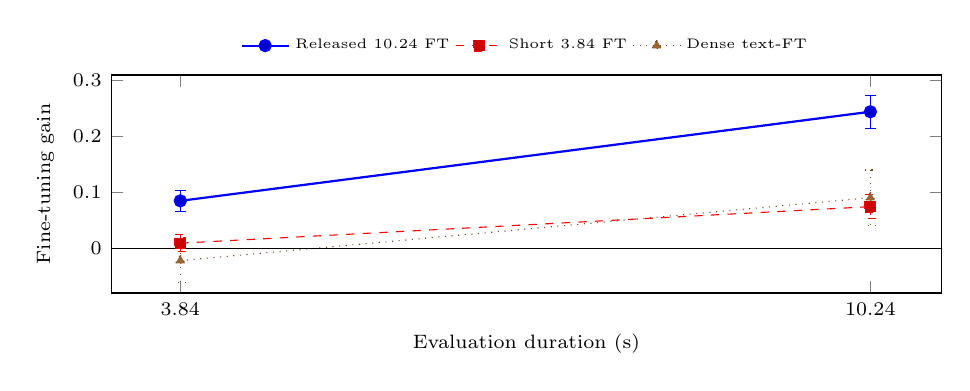
\begin{tikzpicture}
\begin{axis}[
width=\linewidth,height=4.35cm,
xlabel={Evaluation duration (s)},
ylabel={Fine-tuning gain},
xmin=3.2,xmax=10.9,ymin=-0.08,ymax=0.31,
xtick={3.84,10.24},xticklabels={3.84,10.24},
tick label style={font=\scriptsize},label style={font=\scriptsize},
legend style={font=\tiny,draw=none,fill=none,at={(axis description cs:0.5,1.05)},anchor=south,legend columns=-1}]
\addplot+[mark=*,thick,error bars/.cd,y dir=both,y explicit]
coordinates {(3.84,0.0849) +- (0,0.0191) (10.24,0.2443) +- (0,0.0295)};
\addlegendentry{Released $10.24$ FT}
\addplot+[mark=square*,dashed,error bars/.cd,y dir=both,y explicit]
coordinates {(3.84,0.0092) +- (0,0.0152) (10.24,0.0745) +- (0,0.0218)};
\addlegendentry{Short $3.84$ FT}
\addplot+[mark=triangle*,dotted,error bars/.cd,y dir=both,y explicit]
coordinates {(3.84,-0.0220) +- (0,0.0391) (10.24,0.0905) +- (0,0.0496)};
\addlegendentry{Dense text-FT}
\draw (axis cs:3.2,0) -- (axis cs:10.9,0);
\end{axis}
\end{tikzpicture}
\end{minipage}
\caption{Duration dependence and its mechanism test. Left, severity~2 recovery gain rises through the original four-point sweep. The $15.36$\,s follow-up uses $96$ prompts and is shown separately because its matched comparison is a subset of the original sweep. The step from matched $10.24$ to $15.36$\,s is unresolved. Right, a checkpoint fine-tuned at $3.84$\,s still gains more when evaluated at $10.24$\,s. A public dense text-fine-tuned checkpoint shows the same direction, although it is not a recipe-matched causal control.}
\label{fig:duration}
\end{figure*}

\begin{table*}[t]
\centering
\caption{Recovery across duration and domain. All intervals are $95\%$ prompt-bootstrap intervals. Positive KL recovery means that \PFT{} reduces KL to the matched real reference relative to P. Human-CLAP, KL and PANNs sweep rescoring are corroborative analyses.}
\label{tab:evidence}
\setlength{\tabcolsep}{4.2pt}
\begin{tabular}{@{}lcccc@{}}
\toprule
Duration & CLAP $R$ & Human-CLAP $R$ & KL recovery & PANNs capture $R$ \\
\midrule
$3.84$ s & $.085$ $[.066,.105]$ & $.189$ $[.162,.217]$ & $.66$ $[.43,.92]$ & $.19$ $[.06,.32]$ \\
$5.12$ s & $.139$ $[.115,.164]$ & $.278$ $[.243,.314]$ & $1.16$ $[.91,1.41]$ & $.38$ $[.23,.53]$ \\
$7.68$ s & $.201$ $[.175,.227]$ & $.371$ $[.336,.405]$ & $1.95$ $[1.68,2.23]$ & $.76$ $[.61,.91]$ \\
$10.24$ s & $.244$ $[.215,.273]$ & $.375$ $[.340,.409]$ & $2.22$ $[1.92,2.52]$ & $.86$ $[.70,1.02]$ \\
$J$ & $.159$ $[.131,.188]$ & $.185$ $[.151,.220]$ & $1.56$ $[1.20,1.92]$ & $.67$ $[.49,.85]$ \\
\midrule
Domain & $n$ & $R(3.84\,\mathrm{s})$ & $R(10.24\,\mathrm{s})$ & $\rho_{\rm dense}(10.24\,\mathrm{s})$ \\
\midrule
AudioCaps & 192 & $.085$ $[.066,.105]$ & $.244$ $[.215,.273]$ & $.82$ \\
Clotho & 96 & $.098$ $[.072,.125]$ & $.210$ $[.176,.243]$ & $.74$ \\
Hip-hop & 127 & $.026$ $[.008,.044]$ & $.027$ $[.004,.051]$ & $.02^{\dagger}$ \\
\bottomrule
\end{tabular}
\vspace{1pt}
\parbox{0.98\textwidth}{$^{\dagger}$Hip-hop $\rho_{\rm dense}$ uses the original $n=64$ anchor subset. On that subset, dense exceeds its shuffled-caption floor by $.106$ $[.079,.135]$, so the small recovery is not explained by a non-discriminating battery.}
\end{table*}

